\documentclass[conference]{IEEEtran}
\IEEEoverridecommandlockouts
% The preceding line is only needed to identify funding in the first footnote. If that is unneeded, please comment it out.
%Template version as of 6/27/2024

\usepackage{cite}
\usepackage{amsmath,amssymb,amsfonts}
\usepackage{algorithmic}
\usepackage{graphicx}
\usepackage{textcomp}
\usepackage{xcolor}
\usepackage{makecell} % Added to support \makecell in tables
\usepackage{hyperref} % Added to support clickable links
\usepackage{float} % Required for the [H] float option
\def\BibTeX{{\rm B\kern-.05em{\sc i\kern-.025em b}\kern-.08em
    T\kern-.1667em\lower.7ex\hbox{E}\kern-.125emX}}
\begin{document}

\title{Nature Inspired Computing Research Proposal:\\ Transaction Fraud Detection \\ Project Report}

\author{
	\IEEEauthorblockN{Nikita Zagainov}
	\IEEEauthorblockA{
		\textit{Innopolis University}\\
		Innopolis\\
		n.zagainov@innopolis.university
	}
	\and
	\IEEEauthorblockN{Dmitry Tetkin}
	\IEEEauthorblockA{
		\textit{Innopolis University}\\
		Innopolis\\
		d.tetkin@innopolis.university
	}
	\and
	\IEEEauthorblockN{Alisher Kamolov}
	\IEEEauthorblockA{
		\textit{Innopolis University}\\
		Innopolis\\
		a.kamolov@innopolis.university
	}
	\and
	\IEEEauthorblockN{Nikita Tsukanov}
	\IEEEauthorblockA{
		\textit{Innopolis University}\\
		Innopolis\\
		n.tsukanov@innopolis.university
	}
}

\maketitle

\begin{abstract}
	In our work, we propose an approach of using Nature Inspired Computing
	(NIC) algorithm for enhancing the performance of machine learning
	methods in the field of fraud detection. The main goal of our
	research is to provide comprehensive analysis of the application
	of NIC algorithms compared to baseline machine learning methods.
	We also open-source our code, which is available on GitHub
	via the following link: \url{https://github.com/Dmitry057/NIC_Project}
\end{abstract}

\begin{IEEEkeywords}
	Nature Inspired Computing, Fraud Detection, Machine Learning.
\end{IEEEkeywords}

\section{Introduction}
Fraud detection is a critical task in various domains,
including finance, e-commerce, and insurance.
The goal is to identify fraudulent transactions while
minimizing false positives. Traditional methods often rely
on rule-based systems or statistical techniques,
which may not adapt well to evolving fraud patterns.
In recent years, machine learning (ML) approaches have
gained popularity due to their ability to learn from data
and improve over time. However, these methods can be sensitive
to hyperparameters and may require extensive tuning. Furthermore,
real-world data is often imbalanced, with a small percentage of
fraudulent transactions compared to legitimate ones.
This imbalance can lead to biased results and poor performance
of traditional ML algorithms.
In this project, we explore the use of Nature Inspired Computing (NIC)
in combination with machine learning techniques for fraud detection.

\section{Related Work}
Fraud detection has been a subject of extensive research,
and various approaches have been proposed. In this
work, we primarily focus on applications of NIC algorithms
proposed by \cite{github} on publicly available data \cite{dataset}.
The research done by \cite{github}
demonstrates the effectiveness of various NIC algorithms, such as
Firefly Algorithm, Cuckoo Search Algorithm, Bat Algorithm,
Flower Pollination Algorithm, and Grey Wolf Optimizer. However,
the performance of these algorithms was never applied alongside
with novel machine learning methods, such as gradient boosting
algorithms \cite{xgboost, catboost, lightgbm}.

\section{Methodology}
Our experiments aim to evaluate the performance boost achieved
by using NIC algorithms in feature selection in combination with
gradient boosting algorithms.

\subsection{EDA Results}

\begin{figure}[H]
	\centering
	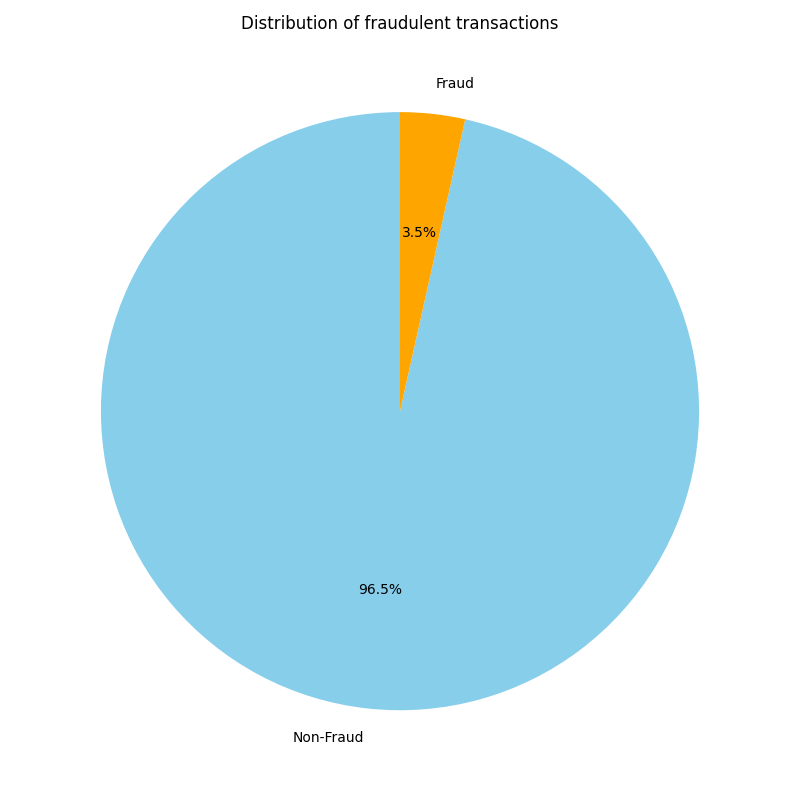
\includegraphics[width=0.4\textwidth]{fraud_pie.png}
	\caption{Distribution of Fraudulent and Non-Fraudulent Transactions}
	\label{fig:fraud_pie}
\end{figure}

We used the publicly available dataset from Kaggle \cite{dataset}
for our experiments. The dataset contains a large number of
transactions, with a small percentage of fraudulent ones
As shown in Figure \ref{fig:fraud_pie}, the dataset is highly
imbalanced, with a significantly smaller proportion of fraudulent
transactions compared to non-fraudulent ones.
This imbalance poses challenges for traditional machine
learning models, which may become biased towards the majority class.
Classical ML algorithms used in \cite{github} are not robust
to this imbalance, leading to poor performance in detecting
fraudulent transactions. However, in our work,
gradient boosting algorithms which utilize ensemble learning
are better suited for handling imbalanced datasets.

\subsection{Experiment Setup}
We setup our experiments as a series of model training and
evaluation steps. We first split the dataset into training and testing
splits, and then we train model on the training split and evaluate on
test split. After that, we apply NIC algorithms to select optimal
features and train a model on the subsample of the features. Then
we measure performance boost achieved by the NIC algorithm with
\texttt{ROC AUC} metric.

\subsection{Models \& NIC Algorithms}
We evaluate two most popular gradient boosting algorithms:
\begin{itemize}
	\item CatBoost \cite{catboost}
	\item LightGBM \cite{lightgbm}
\end{itemize}
Used with the following NIC algorithms:
\begin{itemize}
	\item Firefly Algorithm
	\item Cuckoo Search Algorithm
	\item Bat Algorithm
	\item Flower Pollination Algorithm
	\item Grey Wolf Optimizer
\end{itemize}
All algorithms are taken out of the box from the GitHub repository
\cite{niapy}.

\section{Results}
We present the results of our experiments in Table \ref{tab:results}.

\begin{table}[H]
	\centering
	\caption{ROC AUC of ML models with NIC feature selection}
	\label{tab:results}
	\begin{tabular}{c c c c}
		\hline
		Method & CatBoost & LightGBM & DecisionTree \\
		\hline
		Original Score & 0.886 & 0.912 & 0.818 \\
		Artificial Bee Colony & 0.885 & 0.910 & 0.835 \\
		Cuckoo Search & 0.888 & 0.911 & 0.830 \\
		Bat Algorithm & 0.889 & 0.911 & 0.838 \\
		Firefly Algorithm & 0.887 & 0.910 & 0.836 \\
		Flower Pollination & 0.887 & 0.910 & 0.832 \\
		Grey Wolf Optimizer & 0.890 & \textbf{0.914} & \textbf{0.848} \\
		Particle Swarm & \textbf{0.891} & 0.914 & 0.845 \\
		\end{tabular}
\end{table}

The results show that the performance of decision tree
is increased by applying any algorithm, which supports
results of \cite{github}. However, the performance of gradient
boosting models is improved most of the time.

\section{Conclusion}
In this work, we extend the research done by \cite{github} and
apply NIC algorithms to gradient boosting models. We show that
the performance of simple models, such as Decision Tree, is indeed
improved by applying NIC algorithms. However, the performance
of more advanced models, such as CatBoost and LightGBM, is more
likely to drop after applying feature selection with NIC algorithms.

We hypothesize that the reason for this is that gradient boosting
models are less prone to overfit on large amount of features than
a single-tree model, which is why feature pruning does not
improve the generalization of such models.

As a result of our work, we extended the research done by \cite{github}
and applied NIC algorithms to feature selection for gradient boosting
models and showed that the performance is not always improved,
and we conclude that NIC algorithms for feature selection
might be applicable for Fraud Detection task only in case of
simple models prone to overfitting.

\begin{thebibliography}{00}
	\bibitem{github} GitHub, ``Transacons Fraud Detection,'' Available: \url{https://github.com/pmacinec/transacons-fraud-detecon}.
	\bibitem{dataset} Kaggle, ``IEEE Fraud Detection,'' Available: \url{https://www.kaggle.com/c/ieee-fraud-detecon/overview}.
	\bibitem{xgboost} ArXiv, ``XGBoost: A Scalable Tree Boosting System,'' Available: \url{https://arxiv.org/abs/1603.02754}.
	\bibitem{catboost} ArXiv, ``CatBoost: unbiased boosting with categorical features,'' Available: \url{https://arxiv.org/abs/1706.09516}.
	\bibitem{lightgbm} NeurIPS, ``LightGBM: A Highly Efficient Gradient Boosting Decision Tree,'' Available: \url{https://proceedings.neurips.cc/paper_files/paper/2017/file/6449f44a102fde848669bdd9eb6b76fa-Paper.pdf}.
	\bibitem{niapy} GitHub, ``NiaPy,'' Available: \url{https://github.com/NiaOrg/NiaPy}
\end{thebibliography}

\vspace{12pt}

\end{document}
